\documentclass[10pt]{article}

%------------------------------------------------------
%   PACKAGES
%------------------------------------------------------

% Default 
\usepackage{graphicx}
\usepackage[backend=biber,style=numeric,sorting=ynt]{biblatex}

% Additional
\usepackage{amsmath}
\usepackage{textcomp, gensymb}
\usepackage{placeins}
\usepackage{tabularray} 
\usepackage{xcolor}
\usepackage{placeins}
\usepackage{todonotes}
\newcommand{\td}[1]{\todo[linecolor=blue, backgroundcolor=blue!25,bordercolor=blue, size=\small]{#1}}

\addbibresource{references.bib}

\title{Polarization} 
\author{Rahmanyaz Annyyev, Hikmat Gulaliyev} 
\date{14 March 2024} 

\begin{document}

\maketitle

\begin{abstract}

\end{abstract}

\section{Introduction}

\td{Add some references.}

A wave is a disturbance of a continuous medium that propagates with a fixed shape at constant velocity. If the medium is the \textit{electromagnetic field}, the wave is called an \textit{electromagnetic wave}. 

An electromagnetic wave is comprised of two synchronized oscillations of electric and magnetic fields. Both fields are perpendicular to each other and to the direction of the propagation. Hence, an electromagnetic wave is a \textit{transverse wave}.

An electromagnetic wave can be represented by two perpendicular components. If there is a well-defined relationship between the two components, the wave is said to be \textit{polarized}. An electromagnetic wave that is not polarized is called \textit{unpolarized wave}. The electric field of an unpolarized wave oscillates in all planes perpendicular to the direction of the propagation; it is a mixture of waves with different polarizations. Such a wave can be polarized by passing through a special filter called a \textit{polarizer}.

Essentially, polarization is the phenomenon of restricting, or fixing the oscillation of the electric field of light to a single plane. There are several types of polarization:
\begin{itemize}
  \item Linear polarization. The electric field vector traces a straight line.
  \item Circular polarization. The electric field vector traces a circle.
  \item Elliptical polarization. The electric field vector traces an ellipse.
\end{itemize}

Light is one of the types of electromagnetic waves, and in this experiment, we will study its linear polarization. The primary goal of the experiment is to verify the Malu's law. The equipment is comprised of two polarizers, a laser, a photodetector, an interface, and a rotary motion sensor. The first polarizer will produce linearly polarized light by allowing only the light oscillating in the vertical plane to pass through. The second polarizer will be used to measure the intensity of the light after passing through the first polarizer; it serves as an analyzer.

\begin{figure}[ht]
  \centering
  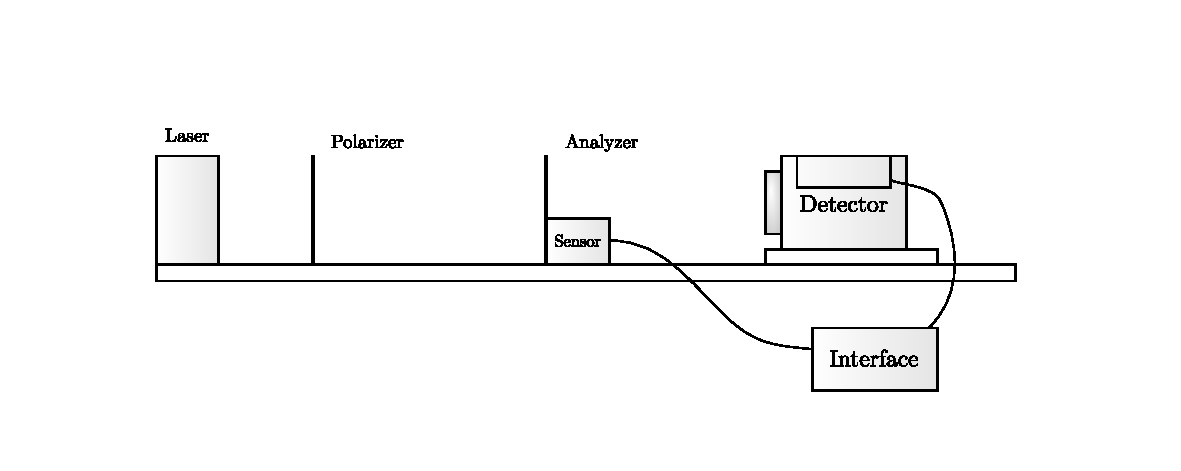
\includegraphics[scale=0.6]{figures/f1.pdf}
  \caption{Experimental setup.}
  \label{fig:1}
\end{figure}

Let's denote the angle between the axis of the first polarizer and axis of the analyzer as $\theta$. If the intensity of the light before passing the analyzer is $I_0$, and the intensity of the light after passing the analyzer is $I$, then the Malu's law states that the intensity of the light after passing the analyzer is given by the equation
\begin{equation}
  I = ...
  \label{eq:1}
\end{equation}
\td{Add the equation for Malu's law. I don't like one in the manual. It doesn't make any sense.}

The procedure of the experiment as follows. First, we turn on the laser and adjust the polarizers so that their axes are parallel. Next, we turn on the interface, namely Pasco\textsuperscript{\textregistered} Xplorer GLX, and start the data collection. We rotate the analyezer by 400\degree. Then we stop the data collection and conclude the experiment.

\section{Data \& Results}

\begin{figure}[ht]
  \centering
  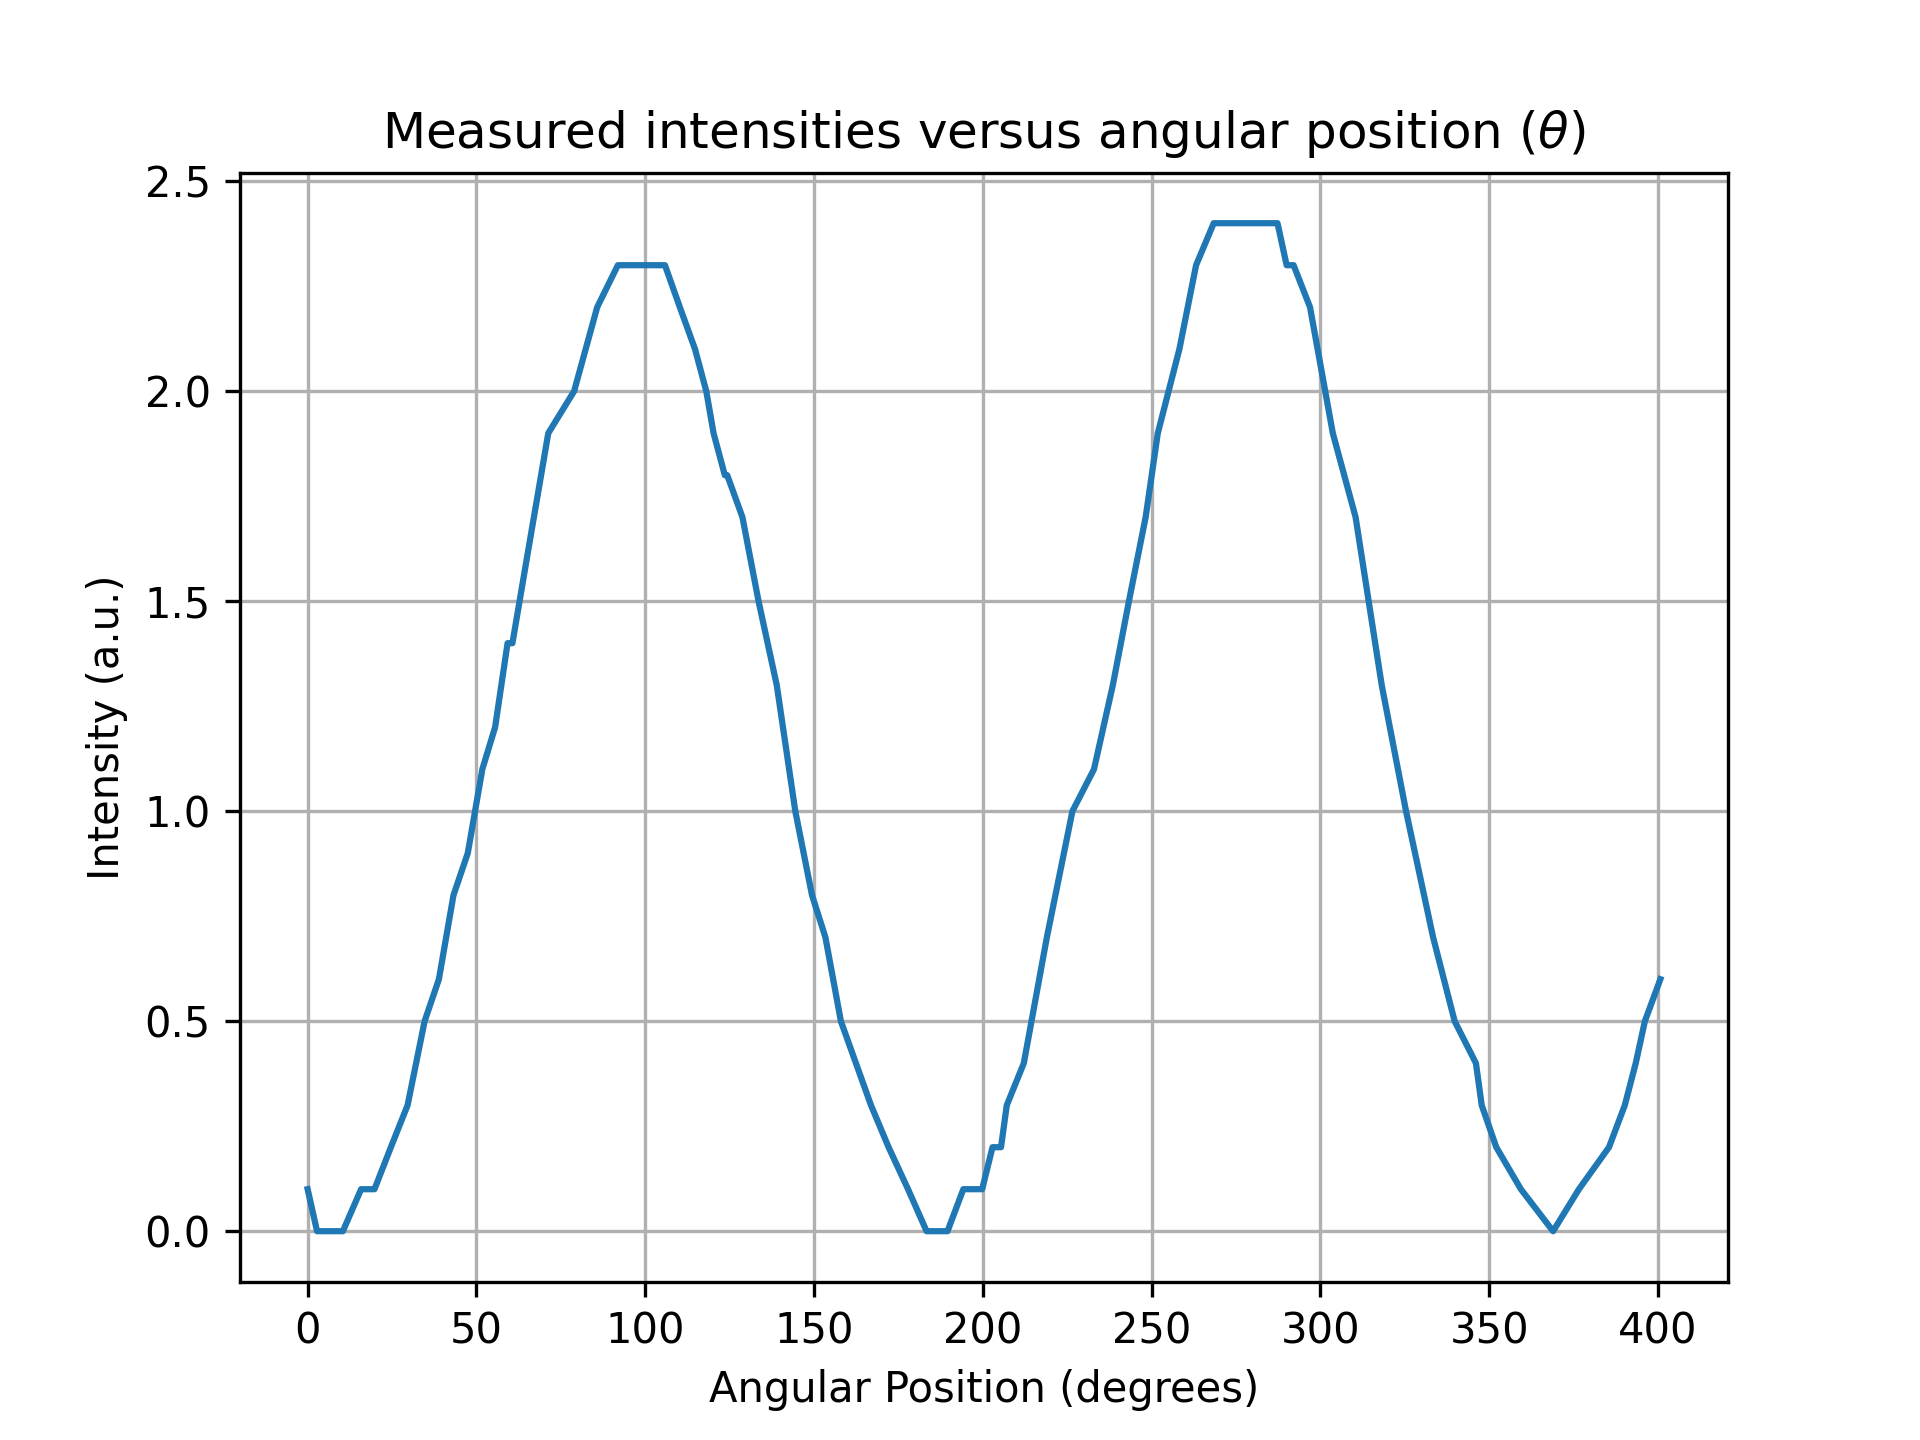
\includegraphics[scale=0.6]{plots/plot1.png}
  \caption{Plot of the intensity of the light after passing the analyzer as a function of the angle between the axes of the polarizer and the analyzer.}
  \label{fig:2}
\end{figure}

\td{The plot looks really funky. Maybe fit the data to the equation given in the manual?}


\td{Don't forget to write about the type of polarization.}
 
\section{Discussion \& Conclusion}

\printbibliography

\end{document}